\section{Logistics}
\label{sec:fdsp-tc-log}
% \cite{bib:docdb8255}

Access to the underground installation area for \dword{dune},   \dword{lbnf}, and \dfirst{jpo} personnel, as well as for  \dword{lbnf} and \dword{dune}  materials and equipment, will be provided solely by the \SI{1500}{m}-deep Ross Shaft. Coordinating transport and ensuring on-time delivery of all items are therefore among the more challenging aspects of the \dword{lbnf} and \dword{dune} endeavor. 
The \dword{jpo} (see \tcchjpo %Volume~\volnumbertc~\voltitletc, Chapter~\ref{ch:tc-jpo} 
of this \dword{tdr}) oversees the \dword{sdwf} where deliveries are received before transport to the Ross Headframe. 

Due to the enormous cost of the \dword{lbnf}-\dword{cf} contracts and the risk of increased construction costs due to delays in delivery of materials, the shaft scheduling must be tightly controlled by \dword{lbnf}-\dword{cf} during construction.
The shaft is outfitted with hoists that control the cage and two skips. The cage is used to transport people, equipment and materials, and the skips to bring up muck and transport over-sized equipment and materials. The \dword{lbnf}-\dword{cf} \dword{cmgc} will coordinate overall usage of the Ross Shaft during this period, until the end of the excavation work. At that  time the \dword{jpo} will take over the management of the shaft usage.


To facilitate the flow of non-\dword{cf} \dword{lbnf} and \dword{dune} materials and equipment to the Ross Headframe, the \dword{jpo} will lease a warehouse facility within a maximum one-day roundtrip\footnote{For purposes of warehouse selection ``one-day roundtrip'' is considered three hours of transportation each way and two hours of unloading and loading at the Ross Headframe.} from \dword{surf} by truck. 
It is expected that the lease of this facility, referred to as the \dword{sdwf}, will include warehouse space, personnel, and a \dword{wms} to inventory all incoming materials and equipment. 
A facility has not yet been selected. 


Most materials and equipment will be shipped to the \dword{sdwf}; \dword{cf} material, and likely cryogenics equipment, are exceptions and will ship directly to \dword{surf}. 
The \dword{sdsd} logistics  organization will (1) receive and inventory all  goods shipped to the \dword{sdwf}, (2) coordinate with the \dword{cf}-\dword{cmgc}  to transport this material to the Ross Headframe in a just-in-time manner, and (3) transport it underground and into the cavern. 
Figure~\ref{fig:logistics-material-flow} shows a high-level overview of the material flow to the Ross Headframe.

 
\begin{dunefigure}[Material flow diagram for \dshort{lbnf} and \dshort{dune}]
{fig:logistics-material-flow}
  {Material flow diagram for \dword{lbnf} and \dword{dune}. }
 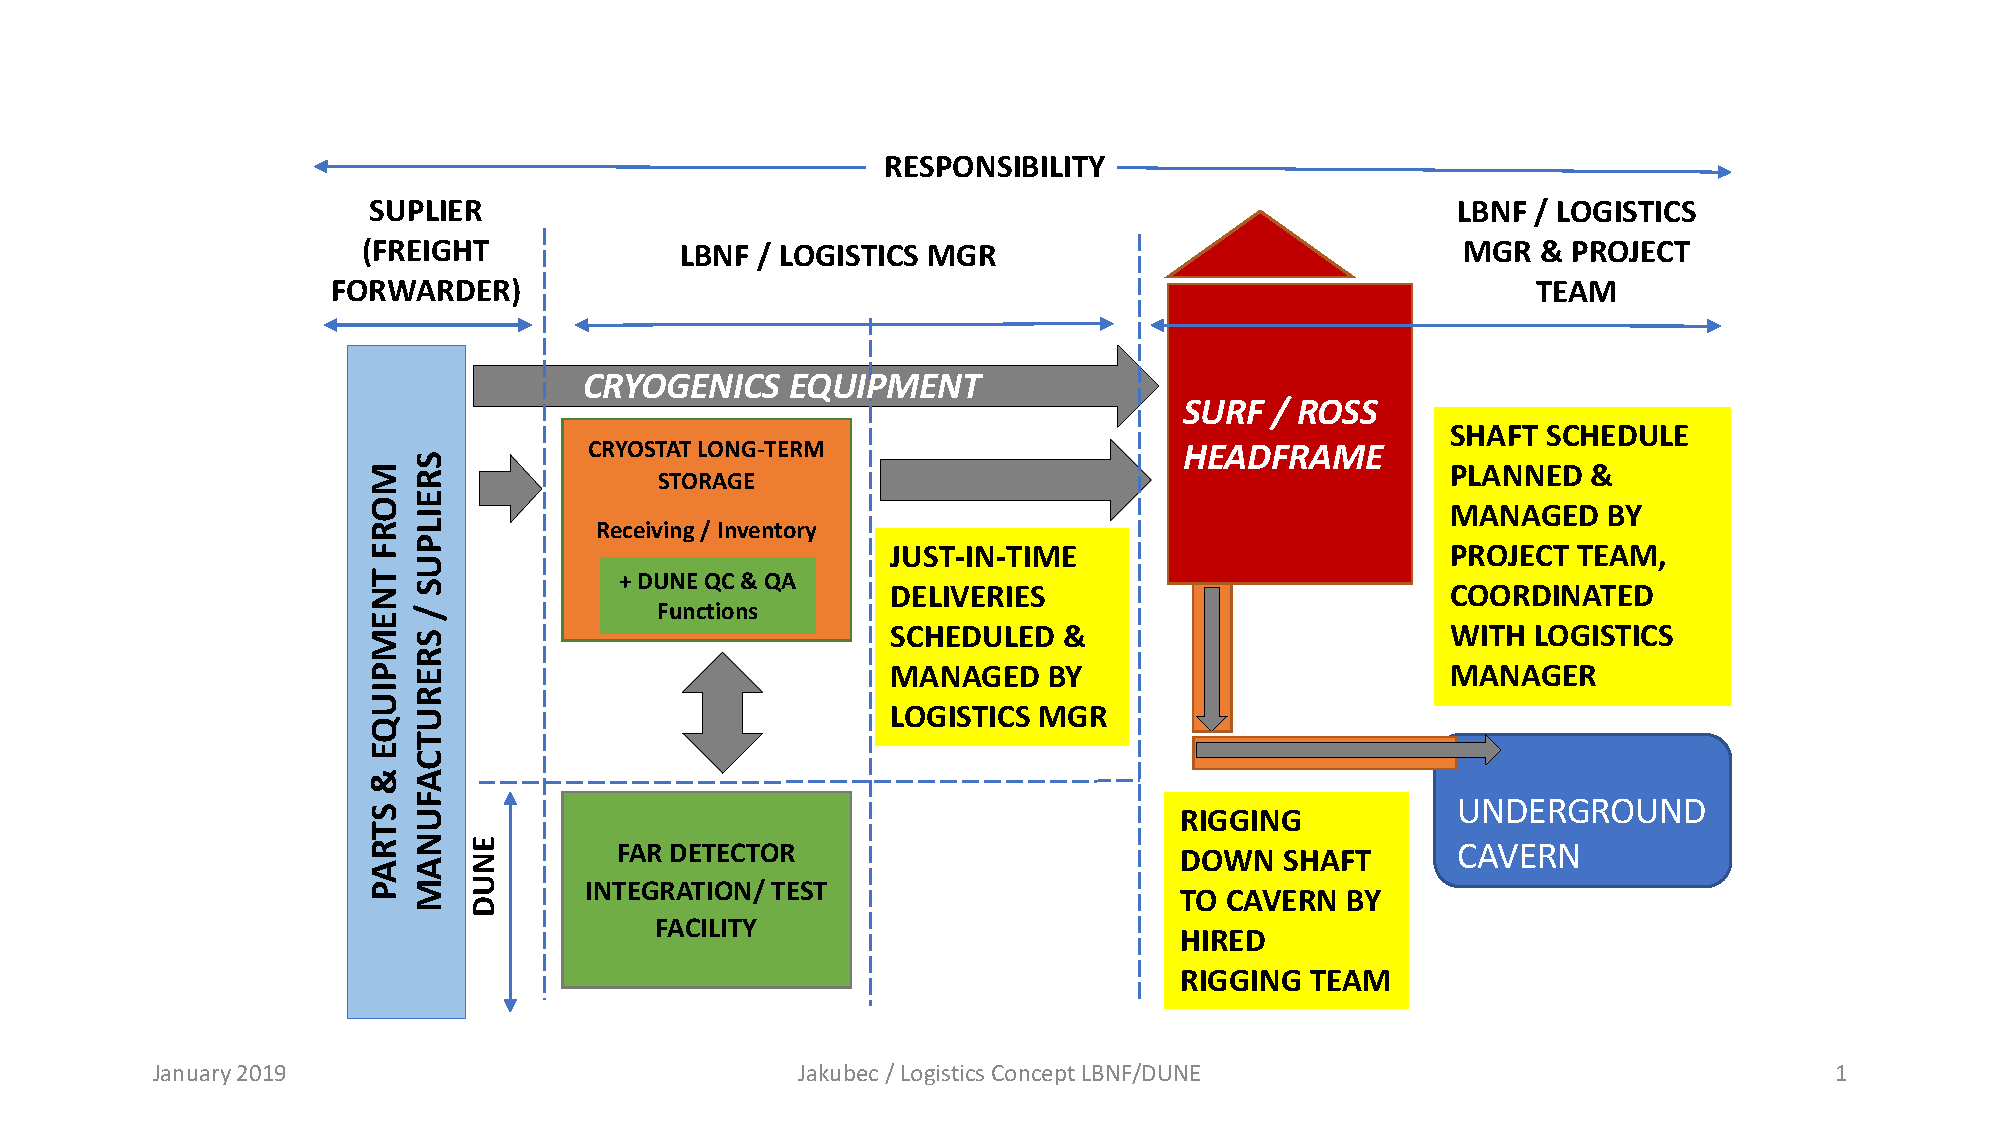
\includegraphics[width=\textwidth]{logistics-material-flow}
\end{dunefigure}

%%%%%%%%%%%%%%%%%%%%%%%%%%%%  
\subsection{Logistics Planning}
\label{sec:fdsp-tc-logPln}

The \dword{jpo}/\dword{sdsd} logistics team oversees transportation of the cryostat (steel, foam, and membrane), the cryogenics system, the \dword{dune} detector components, and all related infrastructure not provided by the \dword{cf}. 
\dword{lbnf} specifically oversees the cryostat and cryogenics system, which \dword{lbnf} will discuss in its %are  discussed in detail in the \dword{lbnf} 
\dword{tdr}. Because \dword{lbnf} materials dominate the logistics, we present a summary of them here, along with an overview of the \dword{dune} materials.  
The steel structure for a single \dword{dune} cryostat requires roughly 1,800 individual steel pieces,  some of which weigh up to \SI{7.5}{t}, as well as \SI{125}{t} of bolts to assemble the steel frame. 
The internal structure for the cryostat, which includes the foam insulation and the thin stainless steel membrane, requires transporting roughly 4,000 boxes of approximate size  \SI{1.5x3.5x1.2}{\meter}. % 1.5 $\times$ 3.5 $\times$ 1.2 m$^3$. 
 The current plan calls for warehousing all these boxes at the \dword{sdwf} before installation begins. 
The logistics operation will require roughly $\SI{5000}{m^2}$ of area available approximately two years before installation of the first \dword{detmodule} begins, to stage construction of the cryostat, cryogenics system, and detector. 
By the time detector components start arriving, most of the cryostat boxes will have been delivered to \dword{surf}, leaving ample space for the detector and the cryogenics components. 
Additional warehouse space may be required if the boxes for the second cryostat arrive before  \dword{detmodule} \#1 installation is complete; a few buildings of the required size are available in the general area around \dword{surf}. 

\begin{dunefigure}
[Simplified model of the Ross Cage]
{fig:fdsp-tc-Cage}
{Simplified Ross Cage model and specifications.}
\parbox{2.1in}{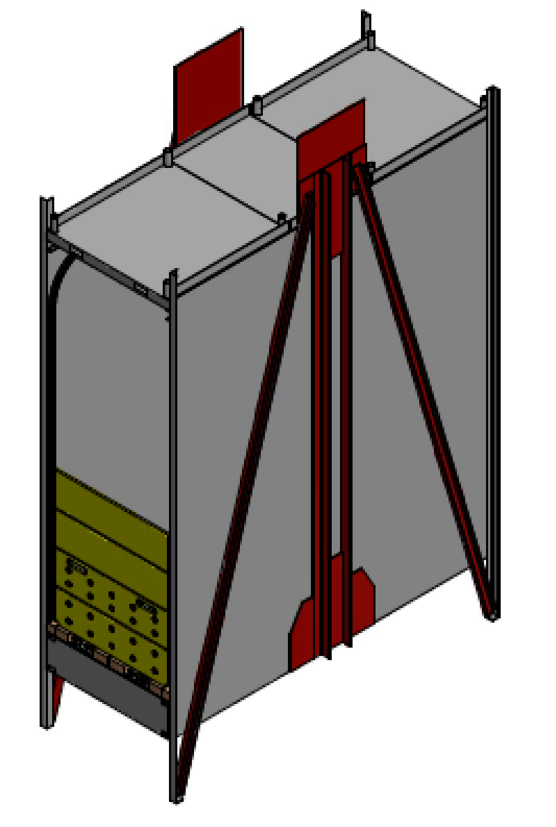
\includegraphics[width=0.3\textwidth]{graphics/Cage-view.pdf}}
\qquad\hspace{10pt}
\begin{minipage}{0.5\textwidth}%
\begin{tabular}{p{3.4cm}p{3.4cm}}        
\multicolumn{2}{c}{Ross Cage Specifications}\\ \toprowrule
Inside height & 3.6 m\\ \colhline
Inside depth  & 3.7 m \\ \colhline
Inside width  & 1.38 m \\ \colhline
Weight limit  &  5,897 kg \\ \colhline
Round trip \newline time & 17 min \newline (incl. unloading) \\ \colhline
\end{tabular}
\end{minipage}
\end{dunefigure}

The \dword{surf} Facility Access Specification~\cite{bib:docdb328} defines the limitations on dimensions and weights for all materials to be transported underground, the most stringent of which are set by the Ross Shaft and Cage. 
It is possible to bring material down the shaft underneath the cage or in the skip compartment  as a slung load, but this is a much slower process and requires careful planning 
and review of detailed procedures for each trip. 
The  \dword{apa}s, for example, require this special handling because they are too tall to fit in the cage. 

Most material will be brought underground inside the cage. Figure~\ref{fig:fdsp-tc-Cage} illustrates the new Ross Cage and summarizes its parameters.  
The roundtrip travel time for the Ross Cage is 17 minutes (actual travel time is \num{3.6} minutes each way), dominated by loading and unloading time.  
Slung loads will require more than an hour round trip.



The Ross Headframe has no loading dock so careful planning of material loading and unloading of shipments is required. 
All materials must arrive at \dword{surf} on a flatbed or curtain-sided chassis, and a forklift will be available for unloading. 
All deliveries, either from the \dword{sdwf} or direct to the Ross Headframe, require (1) coordination with the logistics organization, and (2) minimum two weeks prior notice, per an advance delivery plan.  
 
Logistics will provide to \dword{dune} institutions a shipping manual that  
specifies guidelines on required shipping data and cargo consignment. Adherence to the guidelines will enable the logistics organization to monitor shipping progress and ensure that no delays occur due to incomplete or missing documentation. 


In \dword{pdsp}'s experiences with trans-oceanic international shipping highlighted the need to increase delivery schedule duration beyond the shipper-quoted average, which was sometimes exceeded by as much as three weeks. For \dword{lbnf}/\dword{dune} materials, we will plan shipping and transport so that items arrive in South Dakota a minimum of four weeks before they are expected underground. This buffer will allow sufficient advanced planning for the underground work, with confidence that the installation plan can be maintained.


Sufficient space must be made available at the \dword{sdwf} and in the underground area  to house this material.
The \dword{sdwf} staff will deconsolidate or consolidate arriving cargo into appropriately sized boxes and crates, as needed, for delivery to \dword{surf}, to make the most efficient use of available trucks and the Ross Shaft. 

\begin{dunefigure}[Planned usage of underground space during installation setup]{fig:fdsp-tc-setup}
  {CAD image showing the empty half of the north cavern as used during the installation setup phase of the first \dword{detmodule}.  
The entire cavern is \SI{145}{\meter} long, \SI{20}{\meter} wide, and  \SI{28}{\meter} high; the half shown is therefore approximately \SI{73}{\meter} long.  
Half of this empty space will be used for the cryostat work and half for storage of the detector infrastructure. The material shown outside the cavern must be stored in the \dword{sdwf}.}
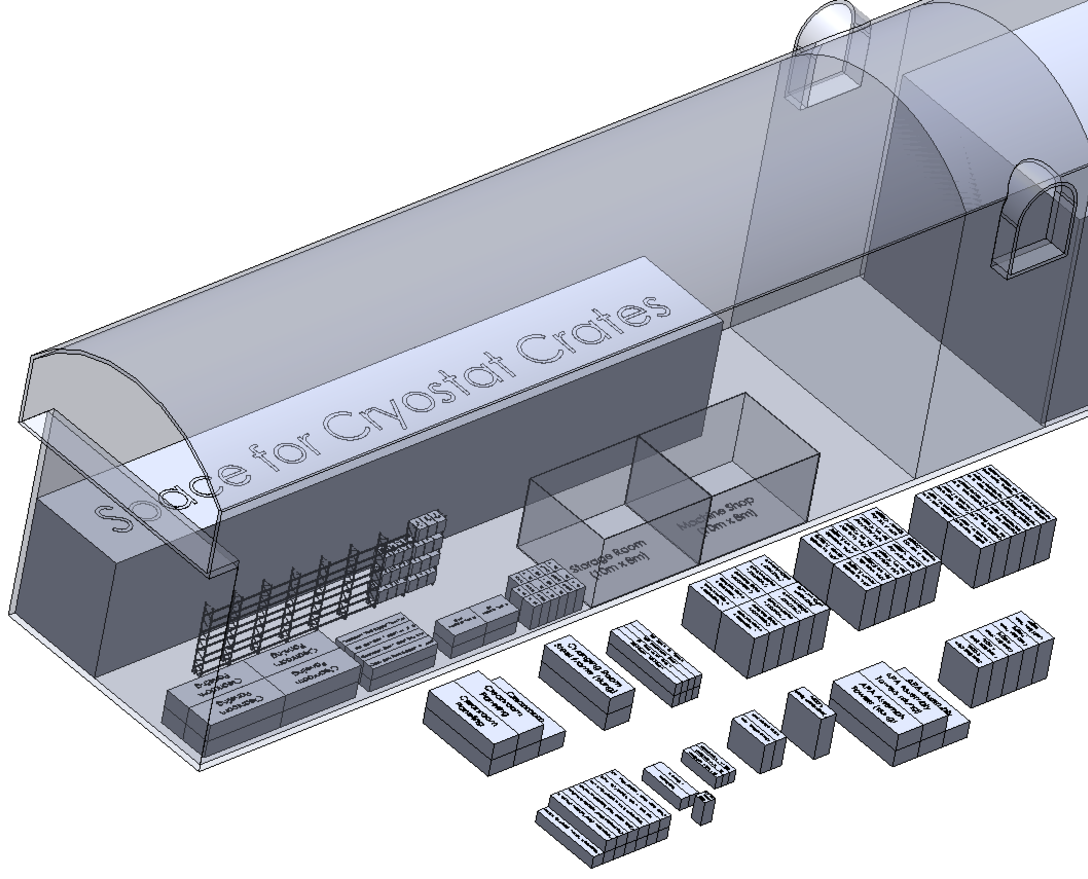
\includegraphics[width=.9\textwidth]{Material-Setup}
\end{dunefigure}


To determine the storage space requirements and how much hoist time must be dedicated to \dword{dune}, a detailed inventory of all  \dword{dune} detector equipment and infrastructure is needed. 
A complete list of materials has been solicited from all consortia and technical coordination. 
The entries in the inventory spreadsheet are organized as \textquotedblleft loads\textquotedblright \ for the Ross Shaft where a load is a crate or set of boxes that will be transported underground in one trip, either in the cage or as a slung load~\cite{bib:docdb8426}. 
Information captured in the load spreadsheet includes the number of  
trips, type of trip (slung load or cage), package dimensions, weight, and type of package (crate, pallet, box, or carton). 

The load list at present predicts 1,600 hoist trips and approximately two  months of cage time, most of which is spread over one year. 
Detector installation (see Figure \ref{fig:high-level-schedule}) for the \dword{spmod} will span two years, so we divide the logistics planning into three phases (summarized in Section~\ref{sec:fdsp-tc-inst}: %{sec:sp-iic-sched}):
 (1) the \dword{cuc} setup phase, (2) the installation setup phase, and (3) the detector installation phase. 
For each phase, a \threed model was generated to show how much material can be stored underground outside the work area and how much material must be stored 
at the \dword{sdwf}, thus setting the surface space requirements. 
The phase with the largest amount of material to transport is the installation setup phase.  
Figure~\ref{fig:fdsp-tc-setup} shows the model of the underground area and the required boxes for surface storage for the first month of this phase. 
The crates outside the cavern were used to estimate \dword{dune}'s storage needs in the surface storage facility. Roughly \SI{1000}{\square\meter} of warehouse space will be needed at this time to buffer \dword{dune} installation equipment.  The \dword{sdwf} will also need space to store up to 150 \dword{apa}s, adding another \SI{700}{\square\meter}. The remaining \SI{3300}{\square\meter} is available for \dword{lbnf} storage. The amount of warehouse space  actually leased can be adjusted to match \dword{lbnf}/\dword{dune} needs, and after the second cryostat construction is complete it will be reduced. 

Managing the hoist and planning all the transport of materials underground is one of the primary responsibilities of the \dword{cmgc}. This task will be challenging and the installation plan with warehouse space on the surface and storage space underground will give critical flexibility in the timing of the delivery of materials. With month-long buffers above and below ground, and a two-week advanced notification of the installation needs, the \dword{cmgc} has freedom to schedule deliveries around the needs of other contractors.


%%%%%%%%%%%%%%%%%%%%%%%%%%%%
\subsection{Logistics Quality Control}
\label{sec:fdsp-tc-log-qaqc}


 
The \dword{pdsp} experience offers a couple of significant lessons regarding logistics.

\begin{enumerate}
\item A central inventory system is essential for tracking  shipments.
\item 
It is important to apply realistic shipping durations based on experience into the overall planning so that work can proceed on a predictable schedule. 
 
\end{enumerate}

The central inventory system  implemented at the \dword{sdwf}  and minimum one-month material buffer are the plans we have in place to prevent repetition of the \dword{pdsp} schedule problems. 
The full list of lessons learned from \dword{pdsp} is in~\cite{bib:docdb8255}. 

Component testing at the \dword{sdwf} is presently not planned, however a \dword{dune} \dword{qc} procedure will be followed to detect any damage incurred during transportation and determine remedial action. Any request from the consortia to perform work in the \dword{sdwf} will be addressed on a case-by-case basis.

In critical cases where the shipping dimensions approach the shaft dimensions, a test transportation using a dummy component will be done. At present the \dword{apa} shipping/transport box is planned to be tested in this fashion.
 
The logistics organization in coordination with the  \dword{sdwf} will inventory all received shipments and  ensure that all materials fit in the Ross Cage, or if a slung load is needed, that the necessary procedures are in place and approved before any material is transported to the Ross Headframe.  
\dword{jpo} representatives will verify that no obvious damage occurred in transport. 

The contribution-in-kind model of this project complicates logistics oversight and inventory control, since components will be delivered from many institutions and from different countries. 
Similarly, during production and testing, \dword{qc} information must be gathered from and made accessible to all collaborators. 
Because of the complexity of the project and the different requirements for \dword{qc} and logistics oversight, two different databases will be used. 
A commercial \dword{wms} will control the inventory process at both the \dword{sdwf} (items both received and shipped) and at \dword{surf} (items received at the Ross Headframe). 
A  separate database, the \dword{dcdb}, will store test and other \dword{qc} data, e.g.,  shipping reports and any reported damage. 
The \dword{wms} will need to provide location and  \dword{qc} information to the \dword{dcdb}, which will ultimately archive both sets of data. 
The \dword{dcdb} has not yet been designed.

Until materials arrive at the \dword{sdwf} (or \dword{surf} if directly shipped), the contributors' freight forwarding system will control the logistics supply chain, which will depend on the contractual circumstances and the contributor's choice. 
However, assuming the shipment is consigned as outlined in the  shipping manual (so that the 
logistics organization has access to the shipping data),  the logistics manager will monitor the cargo progress and step in if a problem arises. 
The \dword{qc} and shipping data flow is shown in Figure~\ref{fig:logistics-data-and-mat-flow}.

 


\begin{dunefigure}[QC and shipping data flow diagram for logistics]{fig:logistics-data-and-mat-flow}
  {\dword{qc} and shipping data flow diagram for the \dword{lbnf} and \dword{dune} logistics.}
 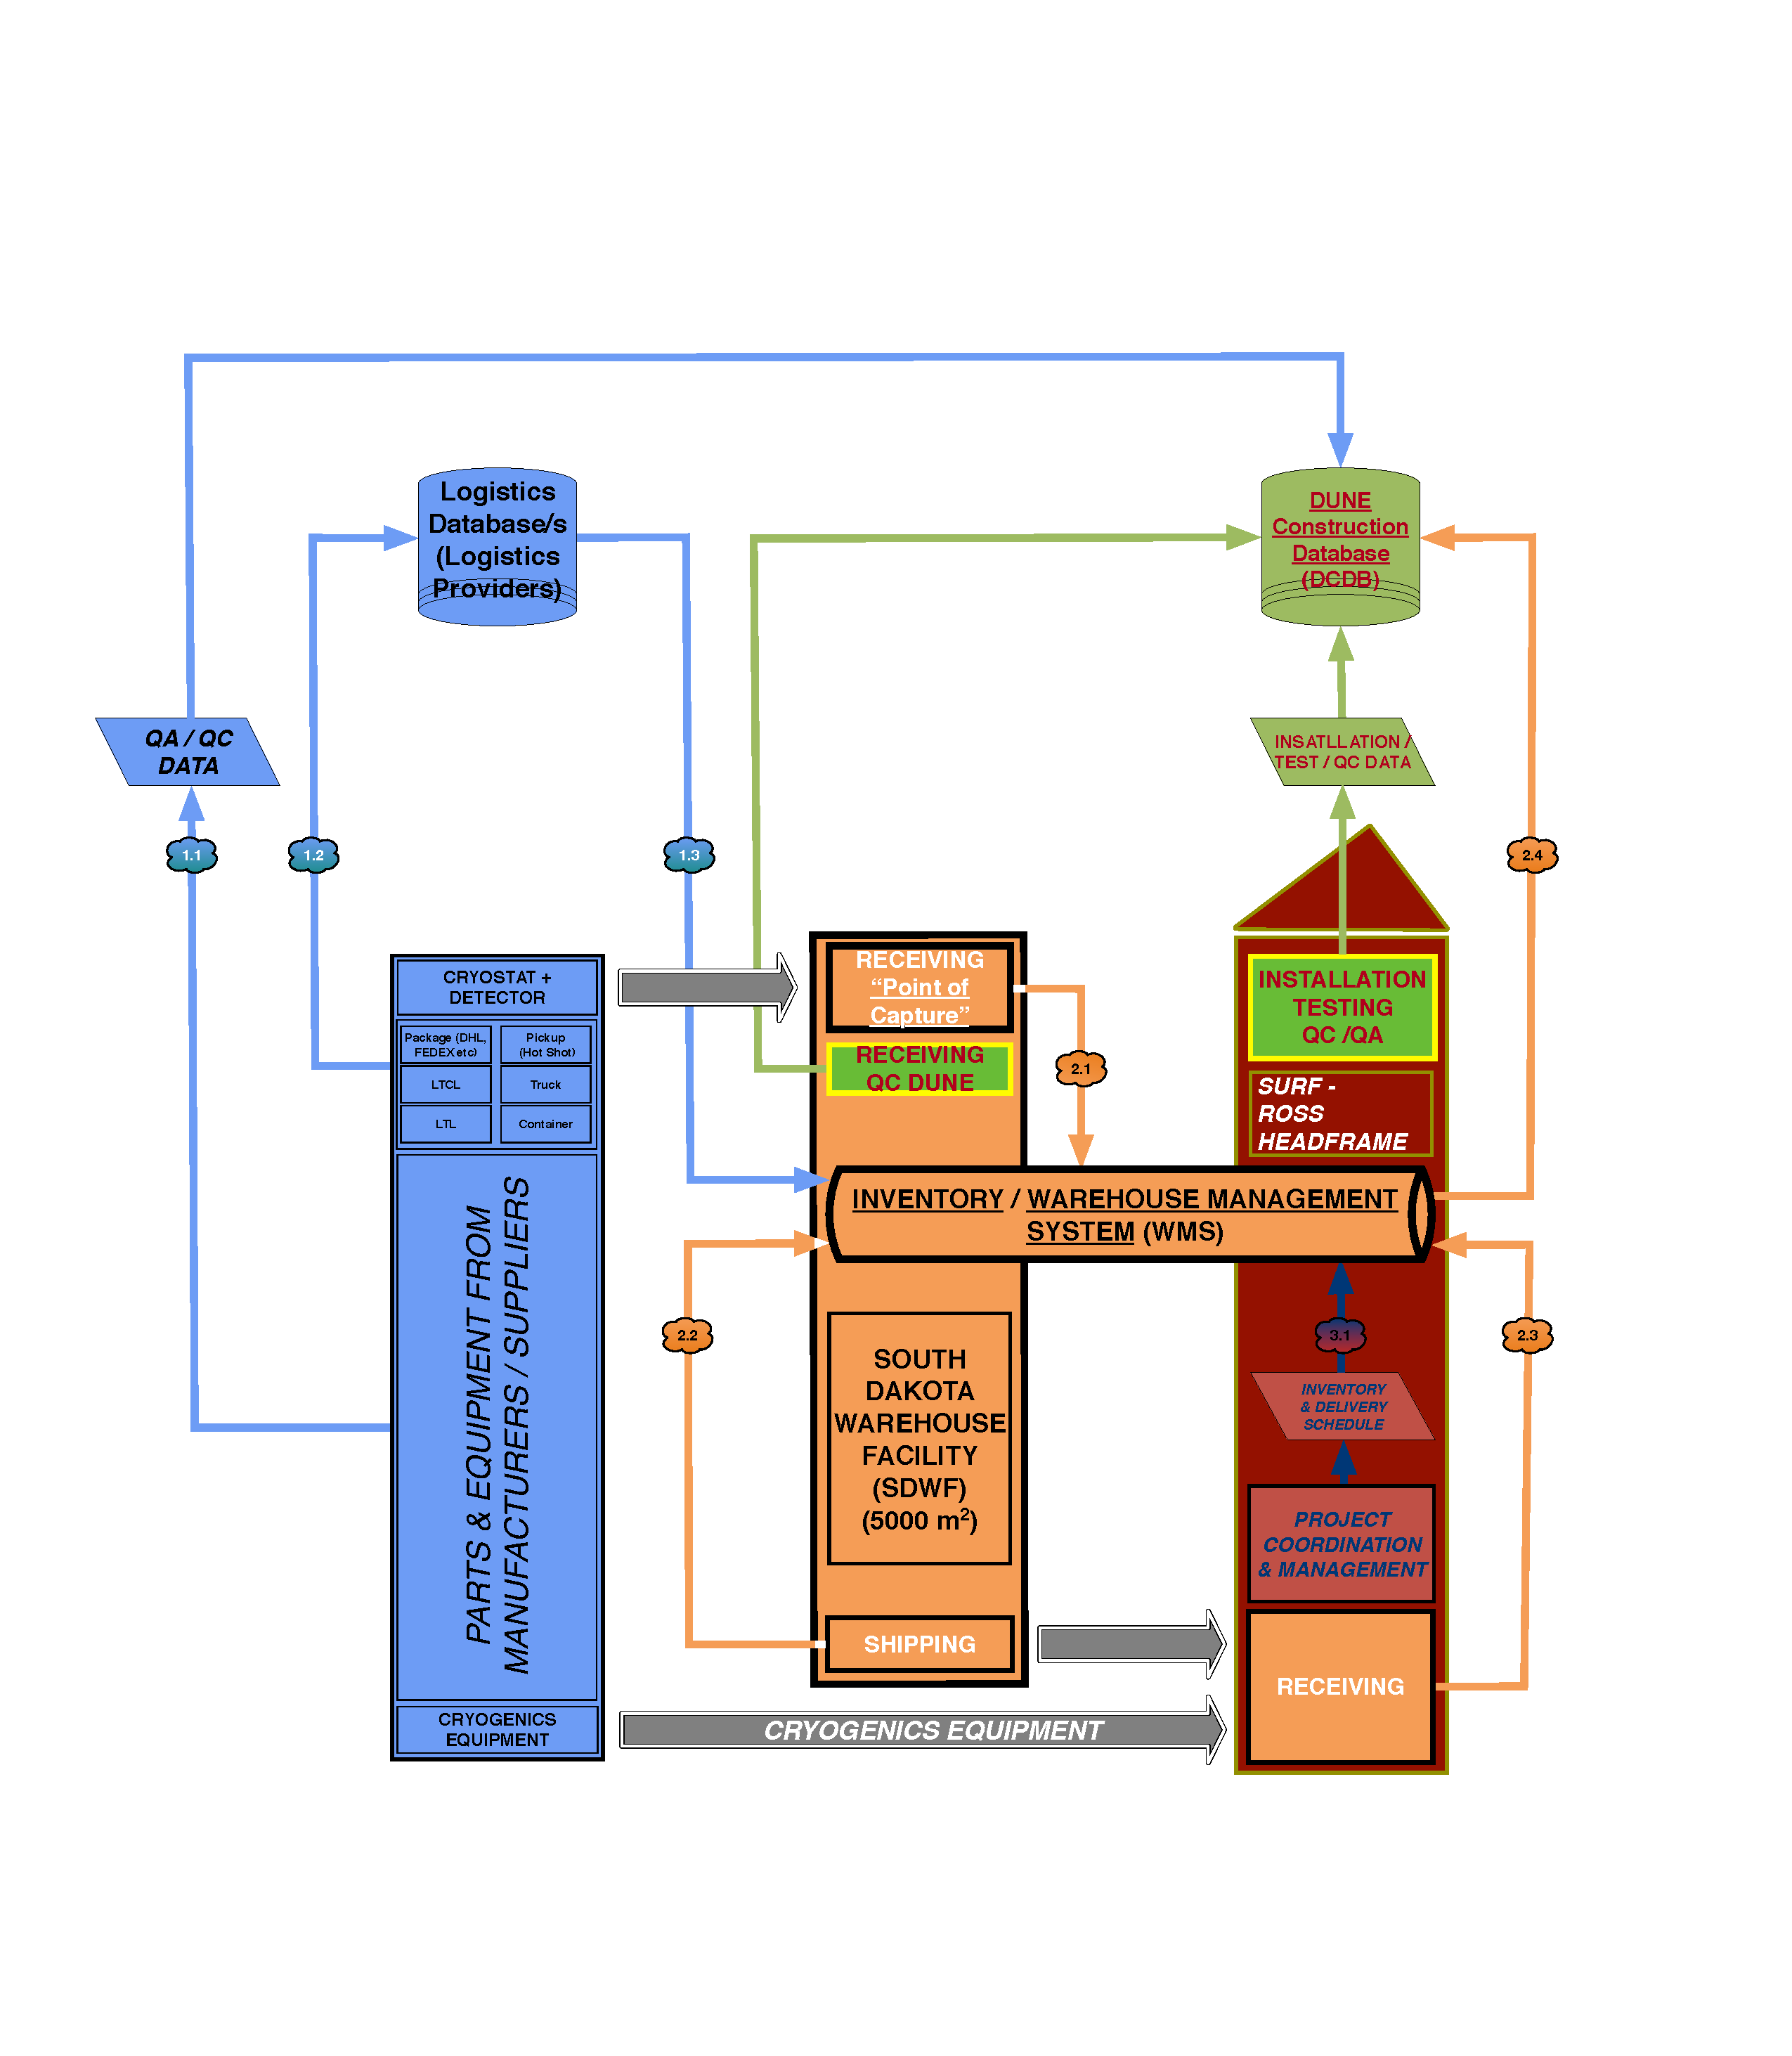
\includegraphics[width=\textwidth]{logistics-data-and-mat-flow}
\end{dunefigure}

 
The \dword{jpo} installation management team will provide a shipping (supply) report to the \dword{sdsd} logistics organization and \dword{sdwf} for scheduling delivery of parts and equipment two weeks in advance of the required delivery date. 
All deliveries will be inventoried upon receipt at the Ross Headframe in the \dword{wms}. 




%%%%%%%%%%%%%%%%%%%%%%%%%%%%
\subsection{Logistics Safety}
\label{sec:fdsp-tc-log-safety}


The \dword{sdwf} will be managed and operated by an independent contractor under the supervision of the \dword{dune} logistics manager. 

The facility will be operated under the contractor's \dword{esh} program, which must conform to federal regulations and will be reviewed by \dword{fnal}'s \dword{esh} management prior to entering a contractual relationship.